\documentclass[a4paper]{article}

\usepackage[english]{babel}
\usepackage[utf8]{inputenc}
\usepackage{amsmath}
\usepackage{graphicx}
\usepackage[colorinlistoftodos]{todonotes}
\usepackage{tikz}
\usepackage{listings}
\usepackage{tkz-berge}
\usepackage{tkz-graph}
\usepackage{numprint}
\usepackage{url}
\usepackage{mathtools}
\DeclarePairedDelimiter{\ceil}{\lceil}{\rceil}

\lstset{frame=single,float=t,basicstyle=\small,caption=,numbers=none}

\title{Testing HPS Features}

\author{Alessandro Edward Galli\\gallia@rpi.edu}

\date{\today}

\begin{document}
\maketitle

\begin{figure}
  \centering
  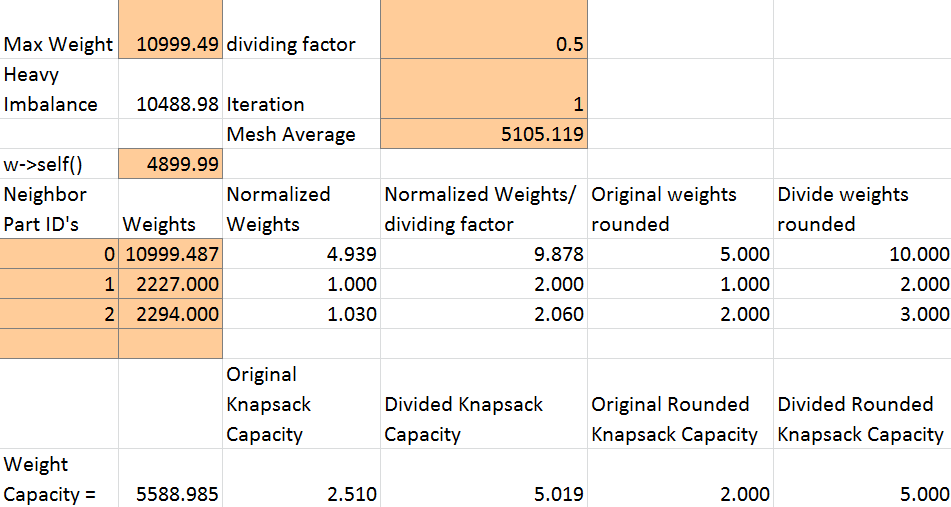
\includegraphics[width=1\textwidth]{knapsack.PNG}
  \caption{\label{fig:knapsacktable}Table of knapsack input calculation for part three of the Torus-4 partition depicted in Figure~\ref{fig:torus4imb}.}
\end{figure} 

\begin{figure}
  \centering
  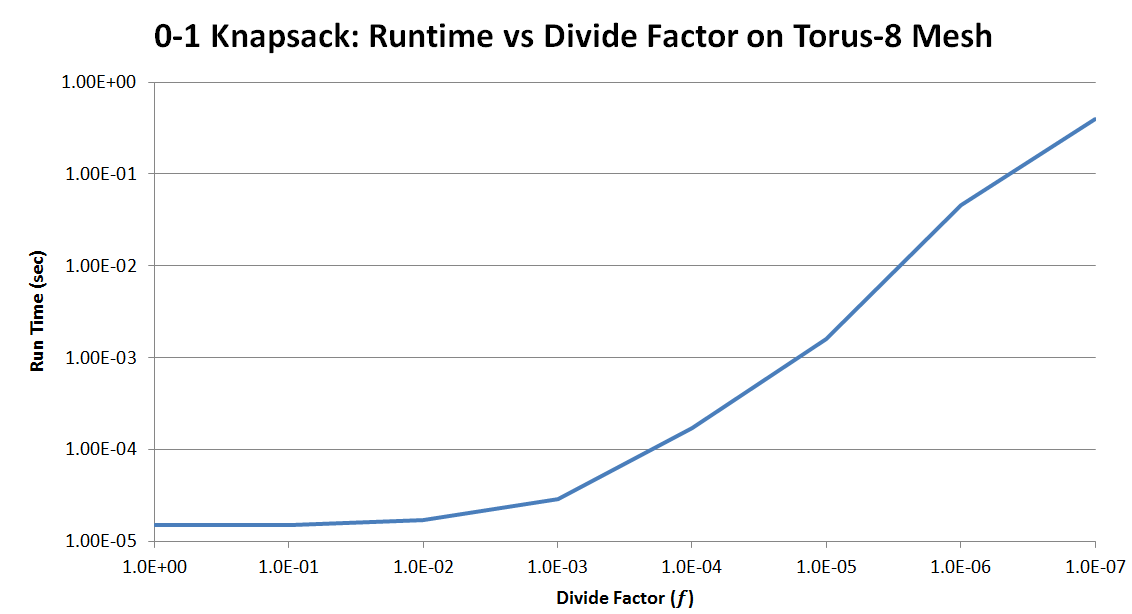
\includegraphics[width=1\textwidth]{Knapsack_Runtime_graph.PNG}
  \caption{\label{fig:knapruntime}0-1 Knapsack Graph on Torus-8}
\end{figure} 

\section{todo}

\begin{itemize}
\item Discuss growth of run-time and memory usage, $O(nf^{-1}W)$, as $f$ changes and how it can be controlled - reference Figure 2.
\item Reference/describe all figures in text - I think the partition graph figures are not discussed.
\end{itemize}

\section{Introduction}

Heavy part splitting, HPS, has three stages: (1) determining what parts can be merged, (2) selecting merging combinations that do not have conflicts, and (3) splitting heavy parts into the newly created empty parts.  Merges are selected by solving the 0-1 Knapsack problem where the items being selected are neighbor parts and the capacity of the Knapsack is defined as $HeavyImbalance$.  The $HeavyImbalance$ is determined by the iterative $chi$, Choose Heavy Imbalance, procedure.  At each iteration the three stages are HPS are performed, but without executing mesh migrations, for the selected value of $HeavyImbalance$.  Currently $chi$ is using a simple scan over a pre-defined range of $HeavyImbalance$ values.  

The Knapsack algorithm uses integer weights for items and the total capacity.  
Since the run time and memory consumption is $O(nW)$ the capacity and weights are normalized to the minumum neighboring part and thus reduces $W$.  
This normalization produces floating point values that are rounded via the floor and ceiling operators, respectively for capacity and weights, to convert them into integer values.  The rounding error is reduced by introducing a scaling reffered to as the `divide factor'.  
The modified weight is defined as follows, $\bar{w} = \frac{w}{minW}*f^{-1}$, where $w$ is the part weight, $minW$ is the minimum neighbor part weight, and $f$ is the divide factor.
For example a weight of .5 will be rounded to 1 and the relative error will be $\centering \frac{1-.5}{0.5}*100 = 100\%$ vs a rounding to .75 where the relative error will be $\frac{1-0.75}{0.5}*100 = 50\%$. 

The amount of error, $\varepsilon$, that the divide factor provides can be defined as \begin{center} $ \varepsilon = (\frac{\ceil{w*f^{-1}}}{\ceil{minW*f^{-1}}} - \frac{w}{minW})*100$ \end{center} 

With this, it can be seen that the divide factor reduces the amount of error from $\varepsilon$ \textless100\% with interger rounding, to $\varepsilon$ \textless$f*100$\% with a divide factor. \todo {CWS - Opinion on setting the error = to a var? - CWS(8/22) where would the var be used in the text?}


This document presents testing that was done on the knapsack problem with the $f$, and MIS Luby, both ported from the old HPS code into parma\_hpsBalance.cc~\cite{scorecGH}. 
Section \ref{sec:knapsack} describes knapsack tests decreasing $f$ and the affect on merge selections. Section \ref{sec:misluby} describes multiple MIS Luby tests.

\section{Knapsack Function}
\label{sec:knapsack}

The table in Figure \ref{fig:knapsacktable} is used to compute the knapsack capacity and item weights after scaling and rounding modifications are applied.  The inputs to the table, highlighted, are described below \todo{CWS, look good? - I made a few tweaks}:
\begin{enumerate}
  \item Self Weight: The weight of the part that is attempting to absorb neighboring parts. 
  \item Neighbor Part Weights: The weights of the neighboring parts.
  \item Divide Factor: 0-1 Knapsack rounding error control. 
  \item $chi$ Iteration: Current $chi$ iteration.
  \item	Mesh Max Weight: The maximum part weight in the mesh.
  \item Mesh Average Weight: The average part weight in the mesh.
\end{enumerate} 
Increasing the iteration of the heavy imbalance decreases the heavy imbalance at the same stepsize as $chi$ would, .1 * the Mesh Average Weight. Modifications to the part weights can be made in the HPS driver test/hps.cc, function applyUnitVtxWeight, by modifying the double, w, on lines 33-36~\cite{scorecGH}. The variable "name" is a reference to the command line argrument that specifies which mesh HPS should balance.

\begin{figure}
\centering
  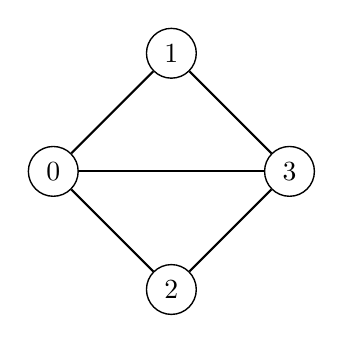
\begin{tikzpicture}
  \SetGraphUnit{1.5}
  \GraphInit[vstyle=Normal]
  \Vertex{0}
  \NOEA(0){1} \SOEA(0){2}
  \SOEA(1){3}
  \Edges(0,1)
  \Edges(0,2)
  \Edges(0,3)
  \Edges(1,3)
  \Edges(2,3)
  \end{tikzpicture}
\caption{Torus 4-Imb Part Neighbor Graph~\cite{meshes}}
\label{fig:torus4imb}
\end{figure}

This knapsack example is used on the Torus4-Imb ~\cite{meshes} mesh provided by SCOREC with two weights being modified: Part 0's weight is multipled by 1.8193, and part 3's weight is multiplied by .804069. This provides an example in which if interger rounding is used, knapsack calculates only one of the neighbor parts as being able to merge into self, where knapsack with the $f$ can recognize that two neighbours can be merged into the self part that we selected. 

\todo[inline, color=green!40]{Talk about what debug setting you should put for output to check if weight edits function also add ref to figure in text}

In Figure \ref{fig:knapsacktable}, the Weight Capacity of part three, 5588.99, is defined as the Heavy Imbalance, 10488.98, minus the self weight, 4899.99. We then calculate that the combined weights of parts one and two are 4521, meaning that they can be merged into self without exceeding the capacity. \todo{CWS, look good? - CWS(8/22) yes}
With $f=1$, we see that the Original Rounded Knapsack Capacity is 2, parts one and two have a value of 1 and 2, respectively, and knapsack can only select one of the parts for merging. 
With $f=.5$, more merges are selected. Here, Parts one and two have a value of 2 and 3, respectively, and since the Divided Rounded Knapsack Capacity is 5, knapsack will select both parts for merging.

\section{MIS Luby Function}
\label{sec:misluby}

\subsection{Introduction}

To test the functionality of MIS Luby, several examples are listed. The examples drive MIS by carefully setting the part weights and the random numbers assigned to merging nets.  The first two examples show that random numbers can be assigned to parts and MIS will produce the expected result. The third example shows that different sized MIS' can be made from the same mesh, and the forth example shows that MIS Luby works over multiple cycles.

These exanples were done by editing the part weights and assigning random numbers to the parts before running MIS. Modifications to the part weights can be done in the file hps.cc, function applyUnitVtxWeight, as shown in lines 33-36~\cite{scorecGH}. The assignment of random numbers is done in 2 steps. First, in the file parma\_hpsBalancer.cc, function generateMisPart, the partId's random numbers are assigned, (intergers only,) while keeping in mind that MIS Luby flows towards smaller numbers. The random number assignment is shown  in lines 172-183~\cite{scorecGH}. Second, in the file parma\_hpsBalancer.cc, function selectMerges, line 204~\cite{scorecGH}, change the last parameter of MIS to true, which tells MIS to use the assigned random numbers you previously specified. To revert to random number assignment by MIS, change the last parameter of selectMerges to false. Lastly, the HeavyImb, if is listed as something other than maxWeight(), can be changed in $chi$ by modifying the hardcoded testW.

For all tests, Part 0 has no mergingNet, and therefore, is always contained in the MIS. Additionally, these are all from the first iteration of $chi$, and these merges are not being forced, but are calculated by knapsack.

\subsection{MIS Testing}

Example 1) Prove that random numbers can be assigned to parts and the results of MIS predicted

\begin{lstlisting}
Torus 4 IMB:
Part Weights:
Part 0) 10999.487
Part 1) 2227
Part 2) 2294
Part 3) 4899.99

Initial HeavyImb = maxWeight()
MergingNets:
1 <- 3
2 <- 3
3 <- 1 , 2

Random Number Assignment:
Part 1) part.randNum = 3
Part 2) part.randNum = 2
Part 3) part.randNum = 1

Predicted: MergeNet 3 will be contained in MIS
Results: Success, MergeNet 3 contained in MIS
\end{lstlisting}
Example 2) Sanity check that different parts can be assigned random numbers and be selected for the set
\begin{lstlisting}
Torus 4 IMB:
Part Weights:
Part 0) 10999.487
Part 1) 2227
Part 2) 2294
Part 3) 4899.99

Initial HeavyImb = maxWeight()
MergingNets:
1 <- 3
2 <- 3
3 <- 1 , 2

Random Number Assignment:
Part 1) part.randNum = 3
Part 2) part.randNum = 1
Part 3) part.randNum = 2

Predicted: MergeNet 2 will be contained in MIS
Results: Success, MergeNet 2 contained in MIS
\end{lstlisting}
\begin{figure}
\centering
  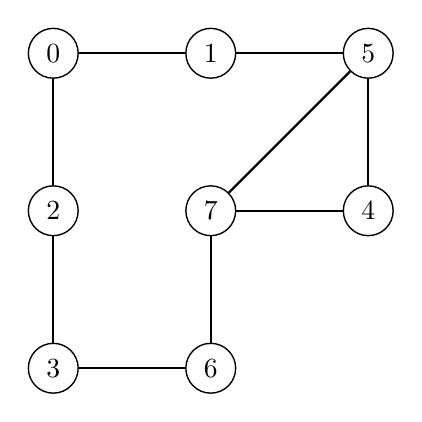
\begin{tikzpicture}
  \SetGraphUnit{2}
  \GraphInit[vstyle=Normal]
  \Vertex{0}
  \EA(0){1} \EA(1){5}
  \SO(0){2} \SO(1){7} \SO(5){4}
  \SO(2){3} \SO(7){6}
  \Edges(0,1) \Edges(1,5)
  \Edges(0,2) \Edges(2,3)
  \Edges(5,7) \Edges(5,4)
  \Edges(7,6) \Edges(3,6)
  \Edges(7,4)
  \end{tikzpicture}
\caption{Torus 8 Part Neighbor Graph ~\cite{meshes}}
\label{fig:torus8}
\end{figure}
Example 3) Show that different sized MIS' can be found on the eight part Torus mesh~\cite{meshes}. \textbf{you might have changed this, I feel it's more important to reference that it's a single mesh - not sure if I changed it previously - CWS(8/22) made some small tweaks}
\begin{lstlisting}
Torus 8:
Part Weights:
Part 0) 3849.6388
Part 1) 2055
Part 2) 2120
Part 3) 1646.7333
Part 4) 2077
Part 5) 2078
Part 6) 2064
Part 7) 2103

Initial HeavyImb = 1.2 * maxWeight()
MergingNets:
1 <- 5 
2 <- 3 
3 <- 6
4 <- 7
5 <- 7
6 <- 7
7 <- 6

Goal: MIS sized 2
Random Number Assignment:
Part 1) part.randNum = 2
Part 2) part.randNum = 2
Part 3) part.randNum = 1
Part 4) part.randNum = 2
Part 5) part.randNum = 1
Part 6) part.randNum = 2
Part 7) part.randNum = 2

Predicted: MergeNets 3 and 5 contained within the MIS
Results: Success, MergeNets 3 and 5 both contained in MIS

Goal: MIS sized 3
Random Number Assignment:
Part 1) part.randNum = 1
Part 2) part.randNum = 1
Part 3) part.randNum = 2
Part 4) part.randNum = 2
Part 5) part.randNum = 2
Part 6) part.randNum = 1
Part 7) part.randNum = 2

Predicted: MergeNets 1, 2, and 6 contained in the MIS.
Results: Success, MergeNets 1, 2, 6 contained in MIS.

Predicted: MIS' of different sizes can be created from the 
  same graph
Results: Success, two MIS created of sizes 2 and 3.
\end{lstlisting}
Example 4) Prove that MIS Luby works over multiple cycles
\begin{lstlisting}
Torus 8:
Part Weights:
Part 0) 3849.6388
Part 1) 2055
Part 2) 2120
Part 3) 1646.7333
Part 4) 2077
Part 5) 2078
Part 6) 2064
Part 7) 2103

Initial HeavyImb = 1.2 * maxWeight()
MergingNets:
1 <- 5 
2 <- 3 
3 <- 6
4 <- 7
5 <- 7
6 <- 7
7 <- 6

Random Number Assignment:
Part 1) part.randNum = 1
Part 2) part.randNum = 3
Part 3) part.randNum = 2
Part 4) part.randNum = 2
Part 5) part.randNum = 2
Part 6) part.randNum = 1
Part 7) part.randNum = 2

Predicted: MergeNets 1, 2, and 6 contained in the MIS
Results: Success, MergeNets 1, 2, and 6 contained in MIS
\end{lstlisting}

\subsection{MIS Tests Conclusion}

All MIS tests were successfully passed and the ported version of MIS works exactly as desired.

\newpage
\bibliographystyle{plain}
\bibliography{references.bib}

\end{document}
